%%%%%%%%%%%%%%%%%%%%%%%%%%%%%%%%%%%%%%%%%
% a0poster Portrait Poster
% LaTeX Template
% Version 1.0 (22/06/13)
%
% The a0poster class was created by:
% Gerlinde Kettl and Matthias Weiser (tex@kettl.de)
% 
% This template has been downloaded from:
% http://www.LaTeXTemplates.com
%
% License:
% CC BY-NC-SA 3.0 (http://creativecommons.org/licenses/by-nc-sa/3.0/)
%
%%%%%%%%%%%%%%%%%%%%%%%%%%%%%%%%%%%%%%%%%

%----------------------------------------------------------------------------------------
%	PACKAGES AND OTHER DOCUMENT CONFIGURATIONS
%----------------------------------------------------------------------------------------

\documentclass[a0,portrait]{a0poster}
\usepackage[utf8]{inputenc}%
\usepackage{multicol} % This is so we can have multiple columns of text side-by-side
\columnsep=60pt % This is the amount of white space between the columns in the poster
\columnseprule=0pt % This is the thickness of the black line between the columns in the poster

\usepackage[svgnames]{xcolor} % Specify colors by their 'svgnames', for a full list of all colors available see here: http://www.latextemplates.com/svgnames-colors
\xdefinecolor{tucol1}{rgb}{1.0 0.5 0.05}
\xdefinecolor{tucol2}{rgb}{0.52,0.72,0.10}
\xdefinecolor{tucol3}{rgb}{0.0 0.0 0.8}
\xdefinecolor{tucol4}{rgb}{0.8 0.8 0}
\xdefinecolor{tucol5}{rgb}{0.8 0 0.8}
\xdefinecolor{tucol6}{rgb}{0 0.8 0.8}
%\xdefinecolor{tucol7}{rgb}{0 0 0.8}
%\xdefinecolor{tucol8}{rgb}{0.8 0 0}
\usepackage{multirow}
\usepackage{times} % Use the times font
%\usepackage{palatino} % Uncomment to use the Palatino font

\usepackage[pdftex]{graphicx} % Required for including images
\graphicspath{{figures/}} % Location of the graphics files
\usepackage{booktabs} % Top and bottom rules for table
\usepackage[font=small,labelfont=bf]{caption} % Required for captions to tables and figures
\usepackage{amsfonts, amsmath, amsthm, amssymb} % For math fonts, symbols and environments
\usepackage{wrapfig} % Allows wrapping text around tables and figures
\usepackage{pgfplots}
\usepackage{bm}
\usepackage{enumitem}

\usepackage{pgfplots}
\usepackage{tikz}
\usetikzlibrary{arrows,positioning,shapes,automata,fit,calc,decorations.pathreplacing,angles,quotes,backgrounds}
\usetikzlibrary{spy}
\usepackage[export]{adjustbox}

\usepackage{booktabs}
\usepackage{tabularx}
\usepackage{array}
\newcolumntype{L}[1]{>{\hsize=#1\hsize\raggedright\arraybackslash}X}
\newcolumntype{R}[1]{>{\hsize=#1\hsize\raggedleft\arraybackslash}X}
\newcolumntype{C}[1]{>{\hsize=#1\hsize\centering\arraybackslash}X}

% Table formatting
\usepackage{multirow}
%\newcommand{\twolinecell}[2][c]{%
%  \begin{tabular}[#1]{@{}c@{}}#2\end{tabular}}

%Define a poster section that writes in bold
\providecommand{\postersection}[1]{
\color{tucol2}
\section*{\sf \huge #1}\Large\sf
\color{Black}
}

% Set standard deviation to boldish
\pgfplotsset{
axis line style={line width=3pt},
/pgfplots/error bars/error bar style={line width=2pt},
/pgfplots/error bars/error mark options={rotate=90,black,mark size=10pt,line width=2pt},
}
\begin{document}


\sf\huge\noindent\color{tucol2}\hspace*{-4mm}
\textbf{\MakeUppercase{Segmentation-based Wordspotting in Handwritten Documents}}\color{Black}
\vspace*{15mm}


\noindent \begin{minipage}[b]{0.7\linewidth}
\LARGE\textbf{Eugen Rusakov and Gernot~A.~Fink\\
\large
(in collaboration with Leonard Rothacker and Hyunho Mo [1])
}\\[0.5cm] 
\Large
Department of Computer Science, TU Dortmund University, Germany
\end{minipage}
\begin{minipage}[t]{0.3\linewidth}
\hspace*{-5cm}

\includegraphics[width=25cm]{tud_logo_rgb.pdf}
\end{minipage}
\vspace*{-20mm}


\begin{multicols}{2}

\postersection{Abstract}
\vspace*{-15mm}
\noindent
Given a user defined query, the task of word spotting is to retrieve a list containing word images that are relevant 
with respect to the query. Typically word spotting methods rank all retrieved word images from a given document 
collection by a certain criterion and sort them by their similarities. These queries can either be word images, 
defined by a user cropping a snipped from a document page or defining a word string which needs to be retrieved. 
As dictionaries can contain many thousands of words, present-day word recognition methods require attribute-based 
classification approaches. Hence, Almazan et al. [2] proposed a word string embedding called 
\emph{Pyramidal Histogram of Characters (PHOC)}, representing the character occurences as binary attributes. 
Retrieval is performed by comparing the predicted PHOC vectors using a certain distance measure, for example 
the cosine similarity. In this work [1], the cosine similarity is replaced by a probabilistic comparison of similarities. 
Lampert et al. [5] proposed a method for a similarity measure called \emph{Direct Attribute Prediction (DAP)}, 
comparing the posteriors instead of distances. 

%\vspace{5cm}

\columnbreak
%
\postersection{Challenges in Handwritten Documents}
\vspace*{-20mm}
%
\begin{tikzpicture}[
	node distance = 5cm,
	auto,
	scale=1.0,
	transform shape,
	triangle/.style = {regular polygon, regular polygon sides=3 },
    node rotated/.style = {rotate=180},
    border rotated/.style = {shape border rotate=180}
	]
	
	\node[
	rounded corners=50pt,  
	%rectangle, draw, 
	minimum height=15cm, 
	minimum width=20cm] 
	(inside)
	at (0,0)
	{	};
	
	% Detector scores
	\node[rounded corners=10pt] at ([xshift=-6em, yshift=0.75em] inside.center) (lrc)
	{
		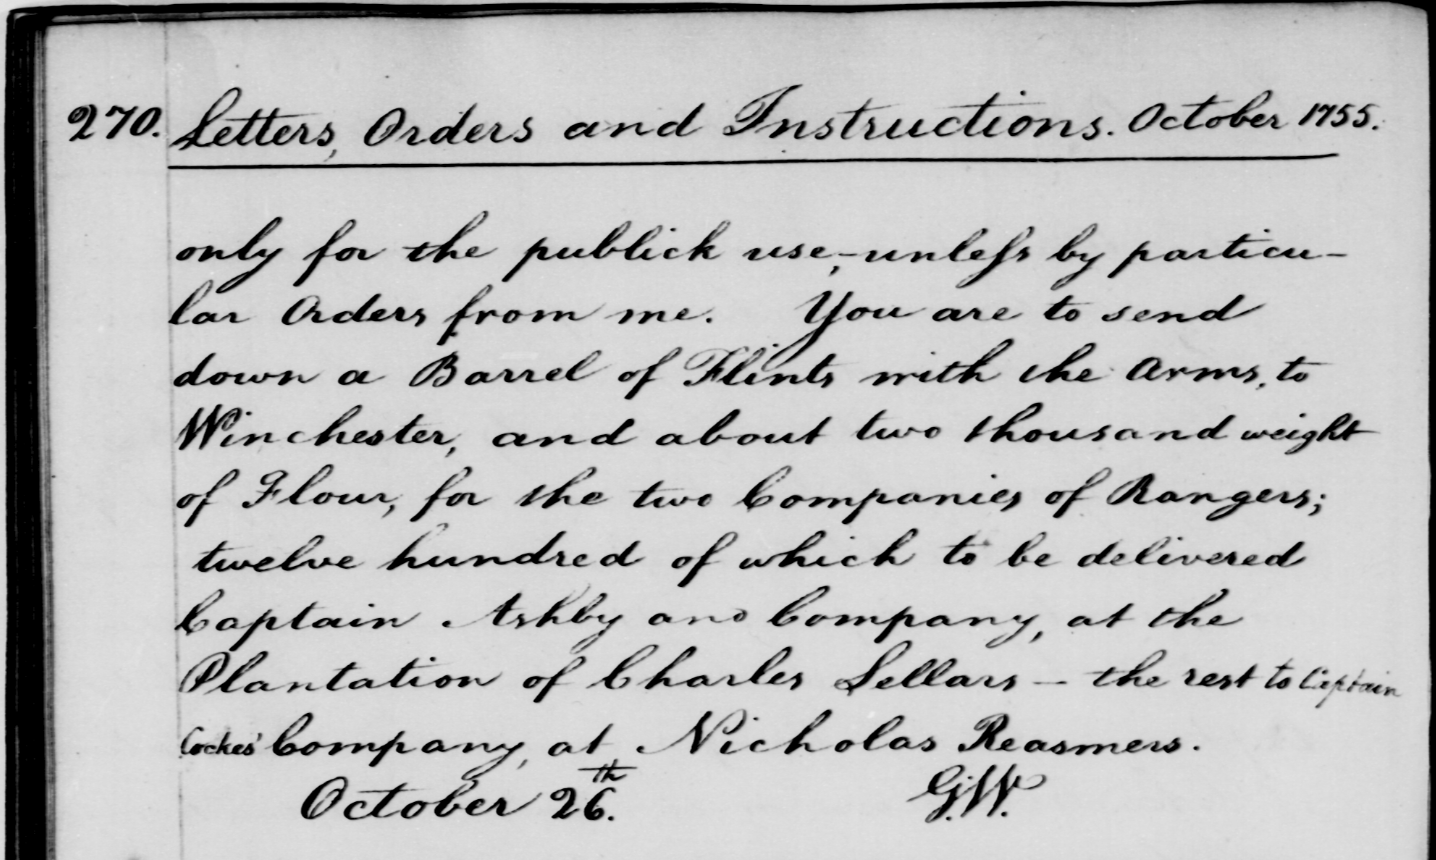
\includegraphics[width=20cm]{images/gw_page_example.png}
	};
	
	\node[rounded corners=10pt] at ([xshift=6em, yshift=3.75em] inside.center) (lrc)
	{
		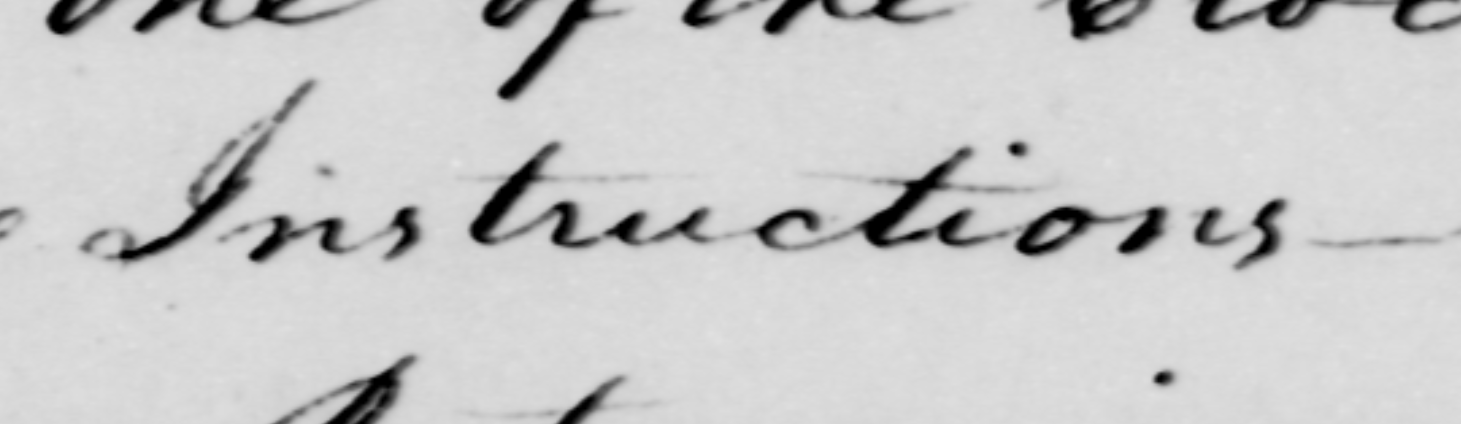
\includegraphics[width=8cm]{images/word_gap.png}
	};
	
	\node[rounded corners=10pt] at ([xshift=6em, yshift=0.75em] inside.center) (lrc)
	{
		
\includegraphics[width=8cm]{images/word_overlap.png}
	};
	
	\node[rounded corners=10pt] at ([xshift=6em, yshift=-2.25em] inside.center) (lrc)
	{
		
\includegraphics[width=8cm]{images/word_overline.png}
	};

\end{tikzpicture}
\vspace{-1cm}
\\
The example above shows the George Washington data set consists of 20 
handwritten document pages. The main challenge in text recognition is 
the amount of word instances (classes). Thus, a attribute-based classification 
approach is required to classify many thousands of words. Especially in historical documents, 
handwritten words can contain faded ink resulting in characters which are not 
fully visible. As the typography of a single writer can contain different lengths for
ascenders and descenders within the same text, different words can overlap.

\end{multicols}

\vspace{-2.5cm}
\postersection{Method}

\vspace*{-30mm}

\begin{tikzpicture}[
	node distance = 1cm,
%	nodes=draw,
	auto,
	scale=1.0,
	transform shape,
	triangle/.style = {regular polygon, regular polygon sides=3 },
	node rotated/.style = {rotate=180},
	border rotated/.style = {shape border rotate=180}
	]
	
	%%%%%%%%%%%%%%%%%%%%%%%%%%%%%%%%%%%%%%%%%%%%%%%%%%%%%%%%%%%%%%%%%%%%%%%%%%%%
	% 4. Word hypotheses
	\node[ 
%	line width=0.2mm,
%	rounded corners=2pt, 
%	rectangle, draw, 
	minimum height=30cm, 
	minimum width=\textwidth]
	at (0,0) 
	(word_spotting)
	{};	
	
% % % Query % % % % % % % % % % % % % % % % % % % % % % % % % % % % % % % % % % % % %

% Query % % % % % % % % % % % % % % % % %
\node[ 
minimum height=1cm, 
minimum width=1cm]
(string_query_label)
at ([xshift=-3em, yshift=-1em] word_spotting.north west)
{
	Query
};

% Query % % % % % % % % % % % % % % % % %
\node[
rounded corners=10pt, 
rectangle, draw,
minimum height=1cm, 
minimum width=1cm]
(string_query)
at ([xshift=0em, yshift=-1em] string_query_label.south)
{
	\textbf{"Captain"}
};

% PHOC % % % % % % % % % % % % % % % % %
\node[
%	rounded corners=3pt, 
%	rectangle, draw,
minimum height=1cm, 
minimum width=1cm]
(phoc_representation)
at ([xshift=12em, yshift=0em] string_query.east)
{
	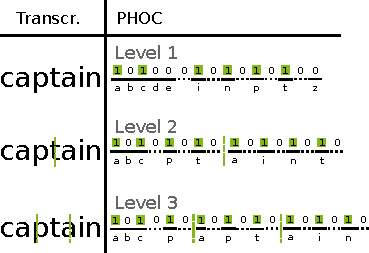
\includegraphics[width=15cm]{gfx/phoc.pdf}
};

\node[
%	rounded corners=3pt, 
%	rectangle, draw,
minimum height=1cm, 
minimum width=1cm]
(phoc_representation_label)
at ([xshift=0em, yshift=0.75em] phoc_representation.north)
{
	\large Word String Embedding
};

\draw[line width=2pt, -stealth] (string_query.east) -- (phoc_representation.west);

% PHOC DAP REPRESENTATION % % % % % % % % % % % % % % % % %
\node[
%	rounded corners=3pt, 
%	rectangle, draw,
minimum height=1cm, 
minimum width=1cm]
(phoc_representation_dap)
at ([xshift=5.5em, yshift=0em] phoc_representation.east)
{
	
\includegraphics[width=0.75cm]{gfx/phoc_vector_q.pdf}
};

\draw[line width=2pt, -stealth] (phoc_representation.east) -- (phoc_representation_dap.west);

\node[
minimum height=1cm, 
minimum width=1cm]
(phoc_vector_q)
at ([xshift=0em, yshift=0.5em] phoc_representation_dap.north)
{
	\normalsize PHOC vector $\mathbf{q}$
};

%%%%% WORD REGIONS %%%%%
	
	\node[
%	rectangle, draw,
	minimum height=15cm, 
	minimum width=8cm]
	(candidate_label_anchor)
	at ([xshift=0em, yshift=-12em] string_query_label.south)
	{
	};
	
	% Word Image % % % % % % % % % % % % % % % % %
	\node[
	align=center,
	minimum height=1cm, 
	minimum width=1cm]
	(candidate_label)
	at ([xshift=0em, yshift=-1em] candidate_label_anchor.north)
	{
		Word Regions
	};
	
	
	% Candidate Captain % % %
	\node[ 
	minimum height=1cm, 
	minimum width=1cm]
	at ([xshift=0em, yshift=-1em] candidate_label.south)
	(captain)
	{
		
\includegraphics[width=7cm]{./gfx/captains.pdf}
	};
	
	% Candidate Captain % % %
	\node[ 
	minimum height=1cm, 
	minimum width=1cm]
	at ([xshift=0em, yshift=-1em] captain.south)
	(captains)
	{
		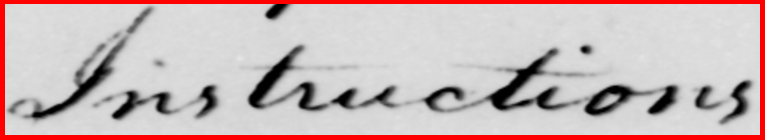
\includegraphics[width=7cm]{./gfx/instructions.pdf}
	};
	
	% Candidate Captain % % %
	\node[ 
	minimum height=1cm, 
	minimum width=1cm]
	at ([xshift=0em, yshift=-1em] captains.south)
	(company)
	{
		
\includegraphics[width=7cm]{./gfx/company.pdf}
	};
	
	% Candidate Captain % % %
	\node[ 
	minimum height=1cm, 
	minimum width=1cm]
	at ([xshift=0em, yshift=-1em] company.south)
	(instructions)
	{
		
\includegraphics[width=7cm]{./gfx/captain.pdf}
	};
	
	
% % % PHOCNet Architecture % % % % % % % % % % % % % % % % % % % % % % % % % % % % %
	\node[ 
%	rounded corners=3pt, 
%	rectangle, draw, 
	minimum height=5cm, 
	minimum width=5cm]
	at ([xshift=11em, yshift=0em] candidate_label_anchor.east)
	(phocnet)
	{
		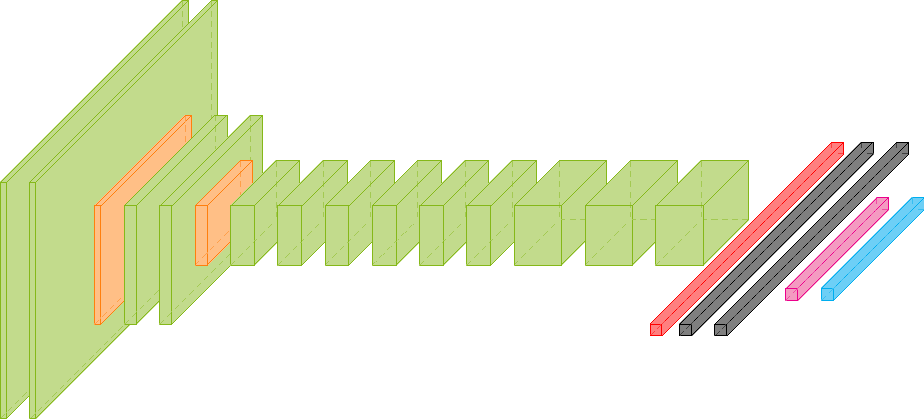
\includegraphics[width=20cm]{gfx/standalone_phocnet_architecture.pdf}
	};

	\node[ 
	minimum height=5cm, 
	minimum width=5cm]
	at ([xshift=0em, yshift=1em] phocnet.north)
	(phocnet_label)
	{
		\large STPP-PHOCNet
	};
	
	\draw[line width=2pt, -stealth] (candidate_label_anchor.east) -- (phocnet.west);
	
	\node[
	minimum height=0cm, 
	minimum width=0cm]
	at ([xshift=-0.2em, yshift=0em] phocnet.east)
	(phocnet_anchor)
	{};
	
	% PHOC DAP REPRESENTATION % % % % % % % % % % % % % % % % %
	\node[
%	rounded corners=3pt, 
%	rectangle, draw,
	minimum height=1cm, 
	minimum width=1cm]
	(phoc_representation_word_image)
	at ([xshift=4em, yshift=0em] phocnet.east)
	{
		
\includegraphics[width=0.75cm]{gfx/phoc_vector_a.pdf}
	};
	
	\draw[line width=2pt, -stealth] (phocnet.east) -- (phoc_representation_word_image.west);
	
	\node[
	minimum height=1cm, 
	minimum width=1cm]
	(phoc_vector_a)
	at ([xshift=0em, yshift=0.5em] phoc_representation_word_image.north)
	{
		\normalsize PHOC vector $\mathbf{a}$
	};
	


% % % Query % % % % % % % % % % % % % % % % % % % % % % % % % % % % % % % % % % % % %

	% Query % % % % % % % % % % % % % % % % %
	\node[ 
	minimum height=1cm, 
	minimum width=1cm]
	(prm_label)
	at ([xshift=5em, yshift=-3em] word_spotting.north)
	{
		Probabilistic Retrieval Model
	};
	
	
	\node[ 
	minimum height=1cm, 
	minimum width=1cm]
	(prm)
	at ([xshift=0em, yshift=-4em] prm_label.south)
	{
		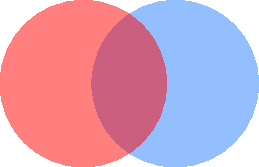
\includegraphics[width=15cm]{gfx/prm.pdf}
	};
	
	\node[ 
	minimum height=1cm, 
	minimum width=1cm]
	(prm_math)
	at ([xshift=0em, yshift=0em] prm)
	{
		\large $\mathbf{p(\mathbf{q}|\mathbf{a})=\prod_{i=1}^{D} q_i^{a_i} \cdot (1 - q_i)^{(1-a_i)}}$
	};
	
	\draw[line width=2pt, -stealth] (phoc_representation_dap) -- (prm);

	\draw[line width=2pt, -stealth] (phoc_representation_word_image) -- (prm);


% % % Retrieval List % % % % % % % % % % % % % % % % % % % % % % % % % %

	\node[
%	rectangle, draw,
	minimum height=13cm, 
	minimum width=8cm]
	(retrieval_list_anchor)
	at ([xshift=7em, yshift=0em] prm.east)
	{
	};
	
	\node[
	align=center,
	minimum height=1cm, 
	minimum width=1cm]
	(retrieval_list_label)
	at ([xshift=0em, yshift=0em] retrieval_list_anchor.north)
	{
		\Large Probability-based\\ 
		\Large Retrieval List
	};
	
	% Candidate Captain % % %
	\node[ 
	minimum height=1cm, 
	minimum width=1cm]
	at ([xshift=0em, yshift=-3em] retrieval_list_anchor.north)
	(captain)
	{
		
\includegraphics[width=7cm]{./gfx/captain.pdf}
	};
	
	% Candidate Captain % % %
	\node[ 
	minimum height=1cm, 
	minimum width=1cm]
	at ([xshift=0em, yshift=-1em] captain.south)
	(captains)
	{
		
\includegraphics[width=7cm]{./gfx/captains.pdf}
	};
	
	% Candidate Captain % % %
	\node[ 
	minimum height=1cm, 
	minimum width=1cm]
	at ([xshift=0em, yshift=-1em] captains.south)
	(company)
	{
		
\includegraphics[width=7cm]{./gfx/company.pdf}
	};
	
	% Candidate Captain % % %
	\node[ 
	minimum height=0cm, 
	minimum width=0cm]
	at ([xshift=0em, yshift=-1em] company.south)
	(instructions)
	{
		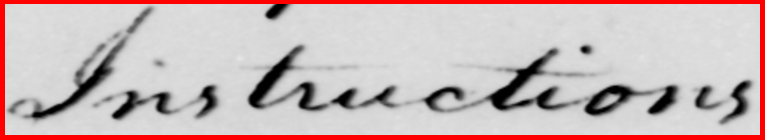
\includegraphics[width=7cm]{./gfx/instructions.pdf}
	};
	
	\draw[line width=2pt, -stealth] (prm) -- (retrieval_list_anchor);
	
\end{tikzpicture}

\vspace*{-6cm}

\begin{multicols}{2}

\postersection{Future Research}

\vspace{-1cm}

\begin{tikzpicture}[
	node distance = 1cm,
	%	nodes=draw,
	auto,
	scale=1.0,
	transform shape,
	triangle/.style = {regular polygon, regular polygon sides=3 },
	node rotated/.style = {rotate=180},
	border rotated/.style = {shape border rotate=180}
	]
	
	% Candidate Captain % % %
	\node[
%	rectangle, draw,
	minimum height=5cm, 
	minimum width=35cm]
	at (0,0)
	(futur_research_box)
	{
	};
	
	% Candidate Captain % % %
	\node[ 
	minimum height=1cm, 
	minimum width=1cm]
%	at ([xshift=5em, yshift=0em] word_spotting.north west)
	at ([xshift=7em, yshift=0em] futur_research_box.west)
	(regions)
	{
		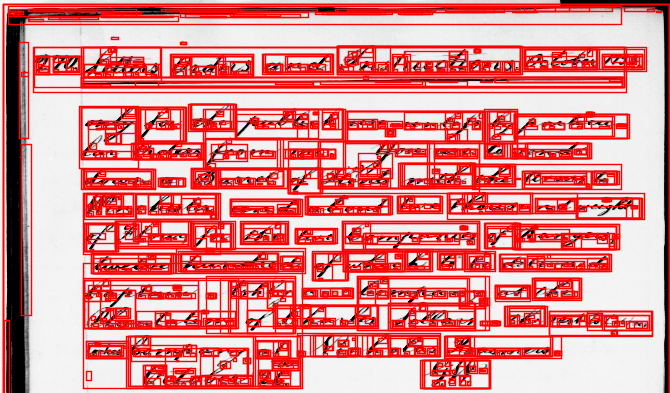
\includegraphics[width=15cm]{./images/sift_regions_top.png}
	};
	
	% Candidate Captain % % %
	\node[ 
	minimum height=1cm, 
	minimum width=1cm]
	at ([xshift=0em, yshift=0.25em] regions.north)
	(regions_label)
	{
		\normalsize Region Proposal Network
	};
	
	% Candidate Captain % % %
	\node[ 
	minimum height=1cm, 
	minimum width=1cm]
	at ([xshift=-7em, yshift=0em] futur_research_box.east)
	(segmentation)
	{
		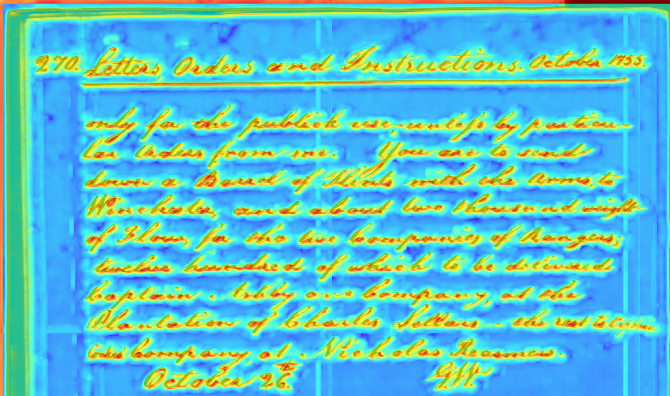
\includegraphics[width=15cm]{./images/semantic_segmentation.png}
	};
	
	% Candidate Captain % % %
	\node[ 
	minimum height=1cm, 
	minimum width=1cm]
	at ([xshift=0em, yshift=0.25em] segmentation.north)
	(segmentation_label)
	{
		\normalsize Attribute-based Segmentation
	};

\end{tikzpicture}
\\
\normalsize
%
The future research is to move from a segmentation-based to the 
segmentation-free word spotting scenario. In contrast to segmentation-based 
word spotting, the words from a document page needs to be detected. 
Here, the challange is to incorporate the knowledge of words (What is a word?) into the 
detection methods. A possible approach could be the region proposal networks, proposing 
regions based on the presumption of the visual apperance of words. Nevertheless, this 
approach lacks of knowledge about words. Another approach could be the semantic segmentation 
based on attribute prediction. Instead of predicting a single class per pixel, a attribute 
vector could be predicted representing the word. The segmentation approach could be 
combined with a sequential model like conditional random fields, hidden markov models, 
or recurrent neural networks.


\columnbreak

\postersection{Results}
%
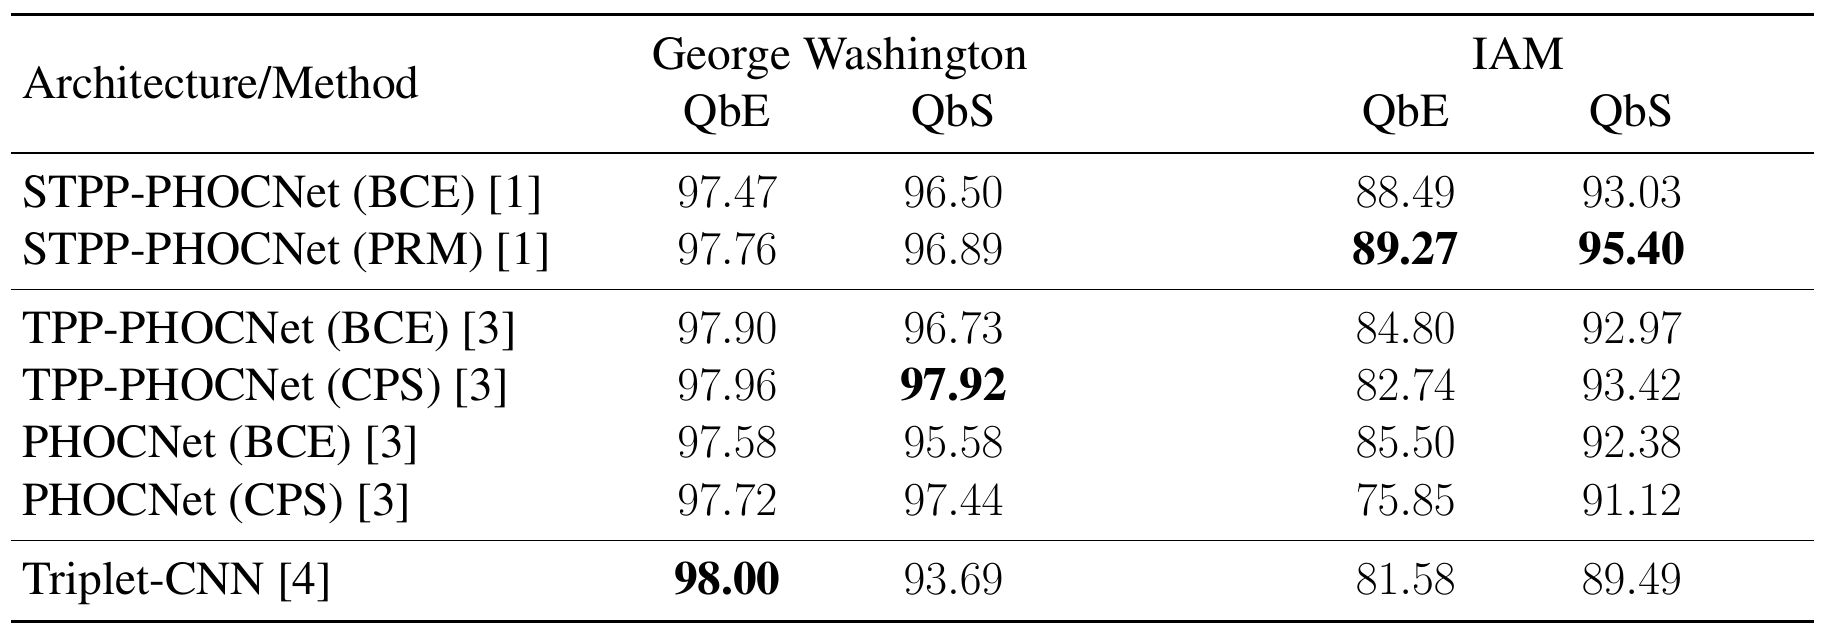
\includegraphics[width=0.48\textwidth]{gfx/results.png}
%
\vspace{1.5cm}
\\
\normalsize
The results are shown on two benchmarks using the \emph{mean Average Precision (mAP)} as evaluation metric 
for the Query-by-Example (QbE) and the Query-by-String (QbS) scenario. 
The method proposed in this work achieves state-of-the-art performance on the larger IAM data set. 
On the George Washington data set all PHOCNet configurations performs nearly equal. As this 
data set is relative small and all recently proposed methods performs close to 100\%, there is 
not much space for improvement.

\end{multicols}
\vspace{-1cm}
\section*{\sf \textbf{References}}
\vspace{-1cm}
\normalsize
\begin{itemize}[leftmargin=1.35em]
 \item[{[1]}] E. Rusakov, L. Rothacker, Hyunho Mo and G. A. Fink, "A Probabilistic Retrieval Model for Word Spotting 
 based on Direct Attribute Prediction", in {\em ICFHR}, 2018.
  
  \item[{[2]}] J. Almazán, A. Gordo, A. Fornés, and E. Valveny, "Word Spotting and Recognition with Embedded Attributes", 
  in {\em TPAMI}, vol. 36, no. 12, pp. 2552-2566, 2014.
  
  \item[{[3]}] S. Sudholt and G. A. Fink, "Attribute CNNs for Word Spotting in Handwritten Documents", 
  in {\em IJDAR}, 2018, to appear.
  
  \item[{[4]}] T. Wilkinson and A. Brun "Semantic and Verbatim Word Spotting using Deep Neural Networks", 
  in {\em ICFHR}, 2016.
  
  \item[{[5]}] C. H. Lampert, H. Nickisch, and S. Harmeling, "Attribute-based Classification for Zero-Shot Visual Object Catigorization", 
  in {\em TPAMI}, vol. 36, no. 3, pp. 453-465, 2014.

\end{itemize}

\end{document}